\documentclass[numbers=noenddot,12pt,a4paper]{scrartcl}
\usepackage[greek,ngerman]{babel}
\usepackage[T1]{fontenc}
\usepackage[utf8]{inputenc}
\usepackage{fullpage}
\usepackage{libertine}
\usepackage{ziffer}
\usepackage{graphicx}
\usepackage{units}
%\usepackage{wasysym}
\usepackage{amsmath}
\usepackage{amssymb}
\usepackage{wrapfig}
\usepackage{esint}
\usepackage{float}
\usepackage{wrapfig}
\usepackage[font=small]{caption}
\usepackage{subcaption}

\renewcommand{\thefigure}{Abb. \arabic{figure}}

\captionsetup[wrapfigure]{name=}
\captionsetup[figure]{name=}
\newcommand{\degree}{^\circ}
\newcommand{\diff}{\textnormal{d}}
\newcommand{\tenpo}[1]{\cdot 10^{#1}}
\newcommand{\greek}[1]{\greektext#1\latintext}
\newcommand{\ix}[1]{_\text{#1}}

\title{Protokoll: Schmitt-Trigger}
\author{Tom Kranz, Philipp Hacker}
\date{\today}

\begin{document}
%\setcounter{page}{2}
%\setcounter{section}{1}
\maketitle
\vspace*{\fill}
\tableofcontents
\vfill
\newpage
\section{Vorbereitung}
\subsection{Schaltskizzen}
\begin{figure}[H]
\centering
\begin{subfigure}[b]{0.49\textwidth}
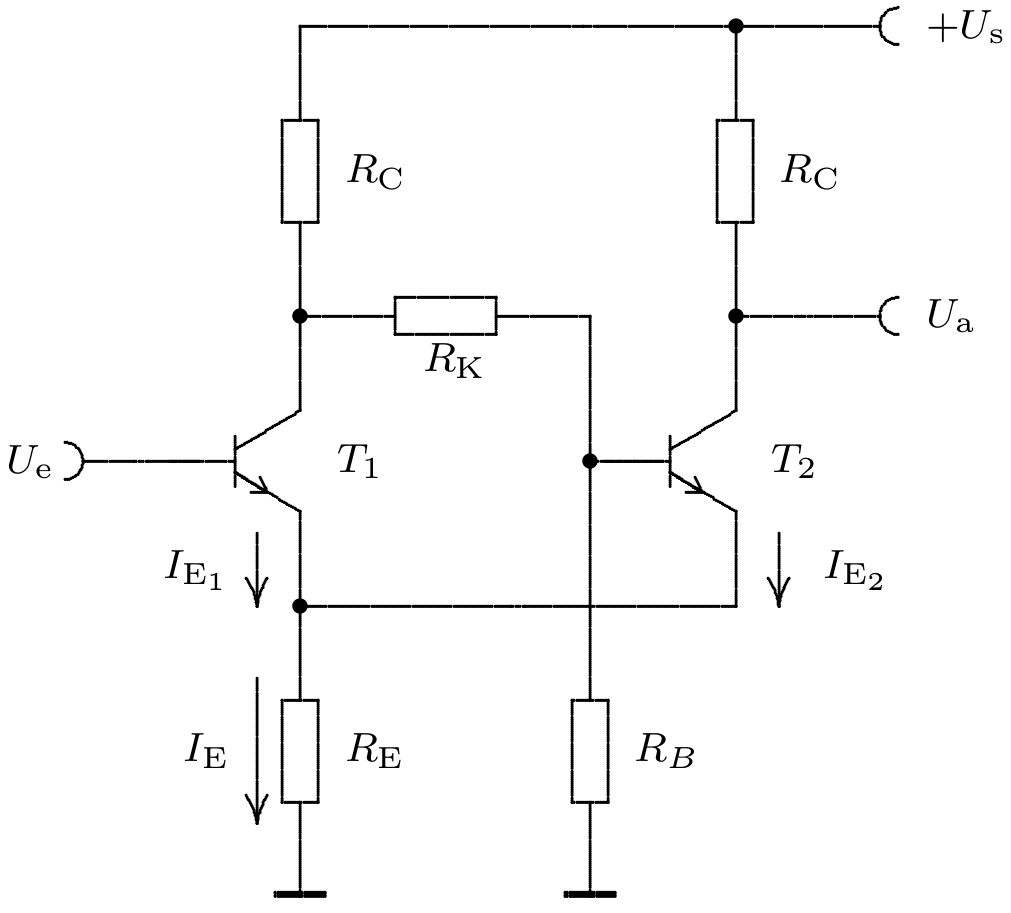
\includegraphics[width=\textwidth]{schaltskizze_st2.png}
\caption{Grundschaltung}
\label{img:grund}
\end{subfigure}
\begin{subfigure}[b]{0.49\textwidth}
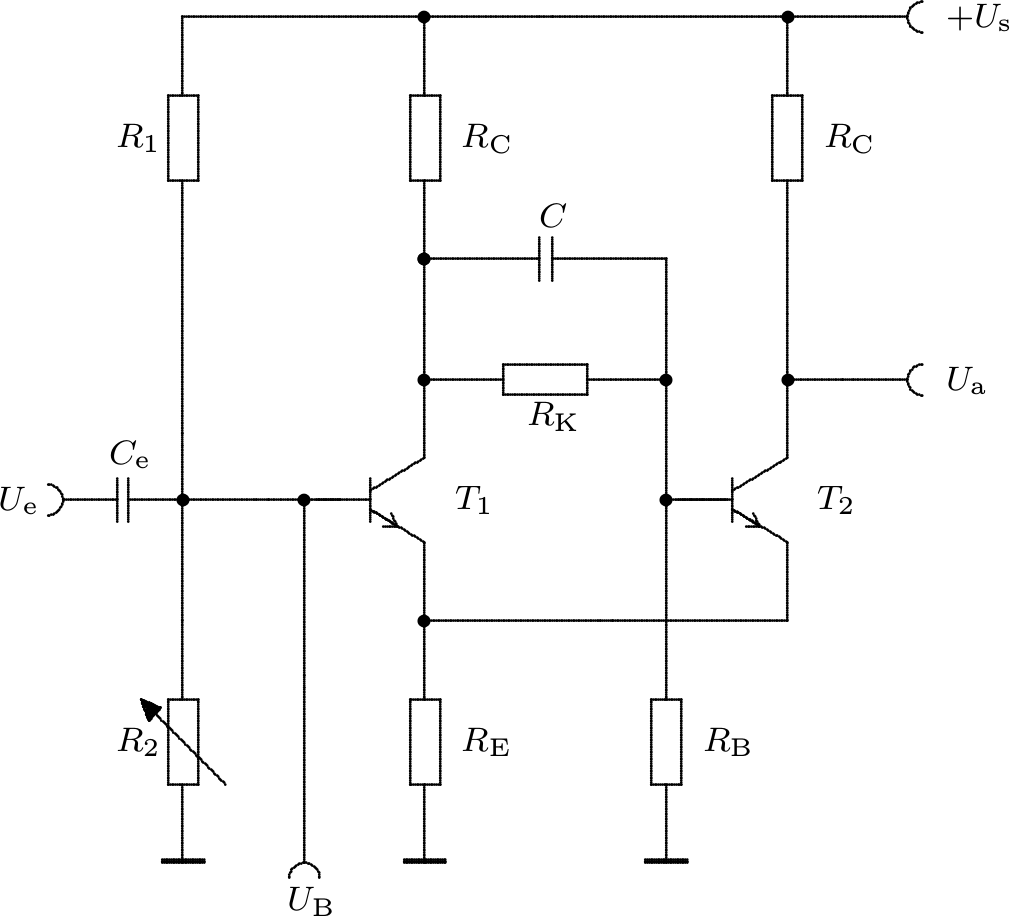
\includegraphics[width=\textwidth]{schaltskizze_st1.png}
\caption{Schaltung mit Modifizierungen $C$, $C\ix{e}$ sowie $R_1$ und $R_2$}
\label{img:mod}
\end{subfigure}
\caption{Schaltbilder zum Schmitt-Trigger}
\end{figure}
\subsection{Dimensionierung}
Grundlage der Dimensionierung stellt dar, dass die Transistoren nur eine gewisse Leistung abgeben können, bevor sie überhitzen, also eine obere Grenze für den Kollektor-Emitter-Strom haben. Die Widerstände $R\ix{C}$ sollten also angemessen groß sein, aber nicht zu groß, da der Basisstrom für $T_2$ zum Durchsteuern ausreichen muss. Auch muss bei der Wahl von $R\ix{C}$ bedacht werden, dass man mit $U\ix{a}$ eventuell ein System besteuern möchte, das $R\ix{C}$ dann als Innenwiderstand seiner Stromquelle sieht. $R\ix{E}$ ist maßgeblich an der Größe des Low-Potentials $U\ix{L}\approx\frac{R\ix{E}}{R\ix{C}+R\ix{E}}\cdot U\ix{S}$ beteiligt, weswegen er kleiner als $R\ix{C}$ gewählt werden sollte, um ein möglichst niedriges $U\ix{L}$ zu erhalten. Des Weiteren muss $R\ix{B}$ groß sein, um den über diesen Weg verschwendeten Strom gering zu halten. Da $R\ix{K}$ mit $R\ix{B}$ einen Spannungsteiler für die Basis-Emitter-Spannung von $T\ix{2}$ bildet, sollte dieser nicht zu groß, für einen angemessenen Basis-Emitter-Strom aber auch nicht zu klein sein. $R_1$ und $R_2$ dienen der Regelung der Schwellspannungen $U_-$ und $U_+$, indem sie eine Basisvorspannung liefern; da hier auch möglichst keine Leistung verloren gehen soll, werden sie groß gewählt. Der Eingangskondensator $C\ix{e}$ bewirkt eine Gleichstromentkopplung -- er kann also weitgehend frei gewählt werden. Schließlich wurden folgende Elemente verbaut:
\begin{table}[H]
\caption{Spezifikationen der verwendeten Bauelemente ($^*$: fest verbaut, hier Nennwert)}
\vspace{-1em}
\begin{align*}
\begin{array}{c|c|c|c|c|c}
R\ix{E} & R\ix{C} & R\ix{B} & R\ix{K} & R_1^* & R_2^* \\ \hline
\unit[99,2]{\Omega} & \unit[556]{\Omega} & \unit[9,94]{k\Omega} & \unit[5,61]{k\Omega} & \unit[5]{k\Omega} & \unit[10]{k\Omega}
\end{array} 
\end{align*}
\end{table}
\subsection{Vorbereitungsaufgaben 1 u. 2}
Schmitt-Trigger werden zur Erzeugung und Flankenversteilerung von Rechteckimpulsfolgen eingesetzt. Somit dienen sie meist der Umwandlung von analogen, beliebigen Signalen $U\ix{e}$ zu \textit{High-} und \textit{Lowpotentialen}, welche binär interpretiert werden können. Weiterhin nutzt man Schmitt-Trigger zur "`Entprellung"' von Schaltern (Auflösen des kurzzeitigen, mehrfachen Öffnens und Schließens eines Tasters) und der Schwingungserzeugung. \\
Die sogenannte Schalthysteresis ist die Differenz aus \textit{High-} und \textit{Low}zustand des ST (\textit{High-} u. \textit{Low}potential fallen nicht zusammen). Sie bestimmt wann das Eingangssignal $U\ix{e}$ als ein Ein- bzw. Ausschalten des Triggers interpretiert wird. Für eben dieses $\Delta U$ gilt näherungsweise
\begin{align}
\Delta U=U_+-U_-\approx\left(U\ix{E}-U\ix{BE;Schw}\right)-\left(U\ix{E}-U\ix{CE;sat}\right)=U\ix{BE;Schw}-U\ix{CE;sat}
\end{align}
\begin{figure}[H]
\centering
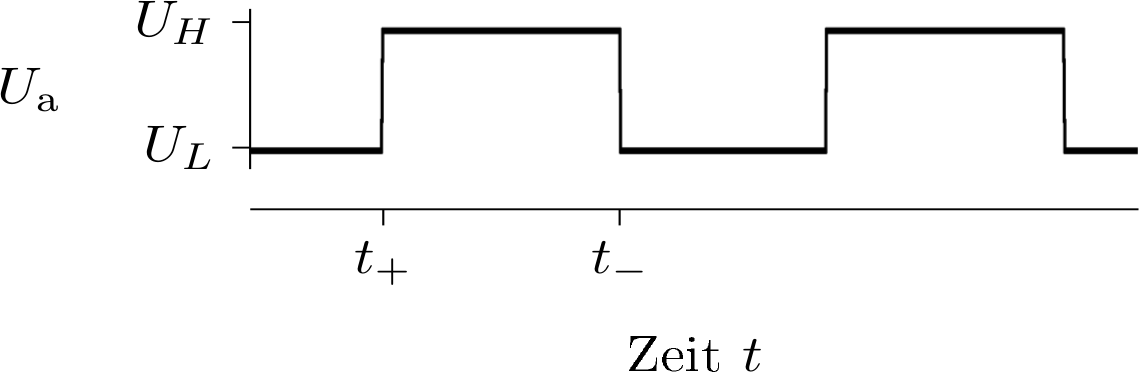
\includegraphics[width=0.55\textwidth]{ausgangssignal.png}
\caption{Ausgangssignal $U\ix{a}$ über $t$ (schematisch; ideal)}
\label{img:signal}
\end{figure}
Die Flankenversteilerung des Ausgangssignals des Schmitt-Triggers (\ref{img:signal}) kann dadurch erreicht werden, dass mittels eines Kondensators $R\ix{K}$ überbrückt wird. Dies hat zur Folge, dass die Spannungssprünge in den Zeitpunkten $t_+$ bzw. $t_-$ vom Kollektor von $T_1$ direkt auf die Basis von $T_2$ übertragen werden können.
\section{Durchführung}
\subsection{Messgeräte}
Die Speisespannung und die verschiedenen Eingangs-Gleichspannungen lieferte das Stromversorgungsgerät \textsc{Tektronix PS 280}, Wechselsignale wurden mit dem Funktionsgenerator \textsc{Tektronix AFG 3022B} erzeugt. Gleichspannungen wurden mit dem Multimeter \textsc{VOLTCRAFTplus VC 920} gemessen, Wechselsignale mit dem Oszilloskop \textsc{Hameg HM1508-2} dargestellt.
\subsection{Versuchsaufgabe 1}
In der Schaltung, welche in \ref{img:grund} gezeigt ist, wurden durch Variation der Eingangsspannung $U\ix{e}$ bis zum Umschlag der Ausgangsspannung $U\ix{a}$ die Schwellspannungen zu $U_+\approx\unit[3,345]{V}$ bzw. $U_-\approx\unit[2,25]{V}$ ermittelt. Die Hysteresis beträgt somit $\Delta U\approx\unit[1,05]{V}$.
\subsection{Versuchsaufgabe 2}
Zur Bestimmung der Abhängigkeit der Kippspannungen von der Speisespannung wurde wie in der vorherigen Messung verfahren. Die Werte der Speisespannung wurden von der Stromversorgung abgelesen. 
\begin{table}[H]
\begin{align*}
\begin{array}{c||c|c|c|c|c|c|c|c|c|c|c}
U\ix{S}\text{ in V} & 5 & 6 & 7 & 8 & 9 & 10 & 11 & 12 & 13 & 14 & 15 \\ \hline
U\ix{+}\text{ in V} & 1,658 & 1,937 & 2,175 & 2,366 & 2,68 & 2,93 & 3,045 & 3,35 & 3,46 & 3,84 & 4,06 \\ \hline
U\ix{-}\text{ in V} & 1,2056 & 1,3756 & 1,48 & 1,61 & 1,7603 & 1,954 & 2,02 & 2,25 & 2,34 & 2,5 & 2,69 \\ 
\end{array}
\end{align*}
\end{table}
\subsection{Versuchsaufgabe 3}
Die Schaltung aus \ref{img:mod} (ohne Kondensator $C$) wurde mit einem Sinussignal der Frequenz $\unit[1]{kHz}$ angesteuert. Ermittelt wurde die kleinste Amplitude des Signals, für welche der ST gerade noch eine Rechteckimpulsfolge erzeugte. Die Einstellung des dafür geeigneten Arbeitspunktes wurde durch die Justierung von $R_2$ realisiert. Für eine Speisespannung von $U\ix{S}=\unit[12]{V}$, sowie der Entkopplungskapazität $C\ix{e}\approx\unit[100]{nF}$ ergab sich die Peak-to-Peak-Spannung zu $V\ix{PP;min}=\unit[1,540]{V}$. Das Potentiometer war dabei auf $R_2=\unit[5,6]{k\Omega}$ gestellt.  
\section{Auswertung}
Der Versuch hat die Funktionen und Eigenschaften des Schmitt-Triggers gezeigt. Es konnte festgestellt werden, dass die Kippspannungen nicht einzig vom Gleichanteil des Eingangssignals, sondern auch von der Speisespannung abhängen. Dies ist in \ref{kuesp} dargestellt. Jedoch basiert eine Berechnung dieser Kippspannungen, wenn überhaupt, auf ungenauen Schätzungen, wie zum Beispiel dem kurz angesprochene Zusammenhang $U_+\approx U\ix{BE;Schw}+\unit[0,5]{V}$. Schließlich hat sich diese Schätzung auch als nicht zutreffend ergeben, was die Notwendigkeit der Vermessung der Schaltung hervorhebt.
\begin{figure}[H]
\centering
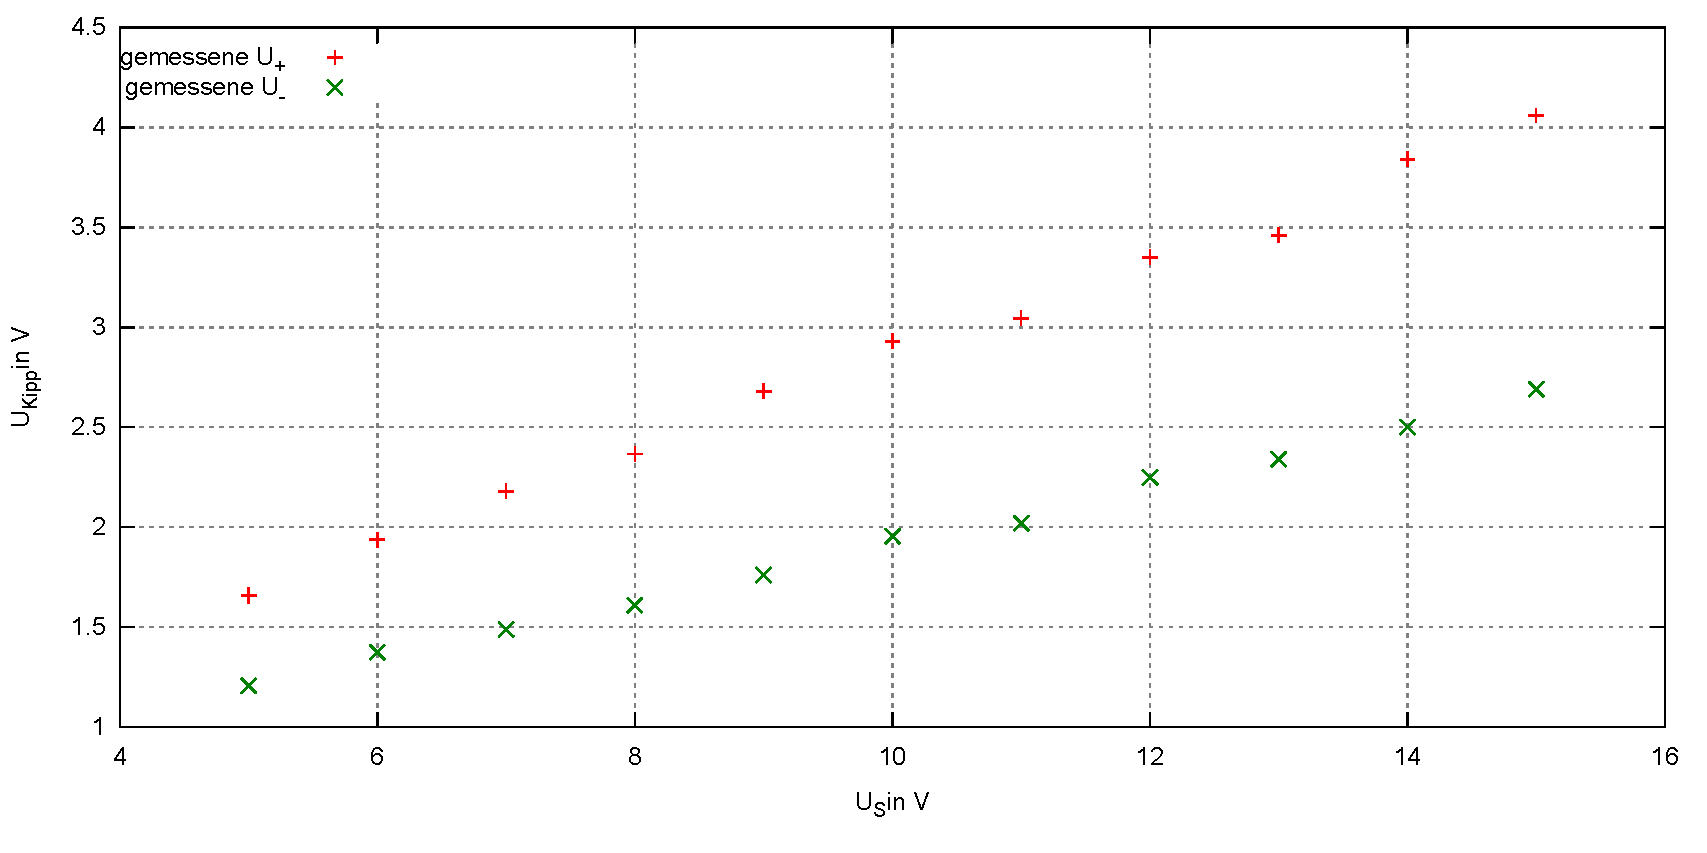
\includegraphics[width=\textwidth]{Messwerte4.pdf}
\caption{Kippspannungen-über-Speisespannung-Diagramm}
\label{kuesp}
\end{figure}
\section{Quellen}
\begin{itemize}
\item \ref{img:grund}, \ref{img:mod}, \ref{img:signal}: "`Elektronikpraktikum"', B. Pompe, 2013
\item \ref{kuesp}: erstellt mit gnuplot, Version 4.6
\end{itemize}
\section{Anhang}
Die originalen Messwert-Aufzeichnungen liegen bei.
\end{document}